B\"ucher, Filme, Spiele: wir haben zahlreiche Wege in andere Welten abzutauchen.
Doch die wenigsten dieser Mittel haben die Mach uns wahrhaft in ihren Bann zu rei{\ss}en, uns einen kalten Schauer \"uber
den R\"ucken zu jagen, uns das Gef\"uhl zu geben, man w\"are wirklich in einer anderen Welt.
Eines dieser Mittel ist der Film, besser noch im Kino und am besten in 3D.
Der erste 3D-Film in einem IMAX-Kino ist schlichtweg unvergesslich.

\begin{center}
    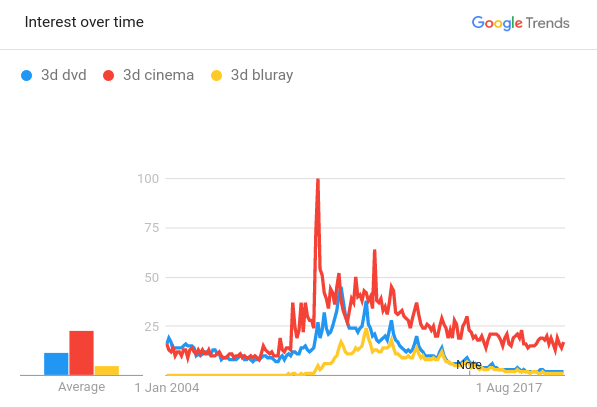
\includegraphics[width=0.66\textwidth]{../img/trends-3d.png}
\end{center}
\noindent\\ Dieses unvergessliche Erlebnis ins eigene Zuhause zu bringen bewegte viele Menschen ihr Heimkino mit 3D-Technologie
auszur\"usten.
3D-Fernseher, 3D-Blu-Ray Player, usw.
Zwar ist dieser 3D-Hype inzwischen recht abgeklungen (siehe Diagramm), doch die Technologien dahinter -insbesondere
das Kodieren mehrerer Ansichten in nur einem Datenstrom (\textit{Multi-View-Coding} oder \texttt{MVC})- sind nach wie
vor
relevant.

\noindent\\ Ein Filmstudio kann zum Beispiel noch beim Schneiden 3D-Effekte probeweise per \texttt{MVC} kodieren,
bevor der Film dann unkomprimiert an das Kino gereicht wird.
Auch im Bereich \"Uberwachung kann stark vom effizienten Kodieren mehrerer Ansichten profitiert werden.
Immerhin befinden sich schlie{\ss}lich mehr als eine Kamera an vielen \"offentlichen Pl\"atzen.

\noindent\\ Die folgende Ausarbeitung pr\"asentiert, wie dreidimensionale Videos entstehen, wahrgenommen werden und
effizient mithilfe von \texttt{H.264} kodiert werden k\"onnen.
Begleitend dazu existiert eine Web-Präsentation als Git-Repository\cite{github}.
